\chapter{Evaluarea modelelor}


Căutarea \textbf{hiperparametrilor optimi} se va realiza pentru fiecare model 
în parte folosind setul de validare. La final, cele mai bune modele 
găsite sunt evaluate într-un mod imparţial pe setul de testare. 

\section{Modele nesupervizate}

\subsection{One Class SVM}

Pentru a exploata capabilităţile de modelare a unei margini de decizie 
neliniare a SVM-urilor, avem nevoie de funcţii kernel care să scufunde
punctele din setul de date într-un spaţiu cu mai multe dimensiuni unde 
să putem găsi mai uşor un hiperplan de separare.

\begin{itemize}
    \item \(K(x, y) = x^T y\) - \textbf{Liniar}
    \item \(K(x, y) = (\gamma x^T y + c)^d\) - \textbf{Polinomial}
    \item \(K(x, y) = \exp\left(-\gamma{\|x - y\|^2}\right)\) - \textbf{Gaussian}
    \item \(K(x, y) = \tanh(\gamma x^T y + c)\) - \textbf{Sigmoid}
\end{itemize}

Un caz particular este kernel-ul \textbf{liniar} care păstrează punctele
în spaţiul iniţial şi încearcă să găsească un hiperplan de separare 
optim la fel ca în cazul clasic fără kernel al SVM-ului.
Acest kernel este nepotrivit în cele mai multe cazuri, mai puţin când 
datele sunt aproape liniar separabile, deci nu ne aşteptăm să performeze
excepţional.

Totuşi, putem exploata eficienţa kernel-ului liniar folosind tehnica de 
optimizare \textbf{Stochastic Gradient Descent} (SGD) împreună cu metoda de aproximare 
\textbf{Nystroem} pentru a aplica o transformare neliniară asupra
datelor de intrare şi apoi să găsim o margine de decizie liniară în noul spaţiu.

SGD este o metodă iterativă relativ simplă ce nu necesită un număr la fel de 
mare de calcule şi nici la fel de multă memorie precum metodele clasice 
de rezolvare a unui sistem de ecuaţii folosind algebră liniară. De aceea, este
potrivită atunci când mărimea setului de date trece de ordinul sutelor de mii,
în ciuda faptului că sacrificăm acurateţea ponderilor estimate.

Metoda Nystroem aproximează matricea kernel pentru o anumită funcţie kernel dată,
folosind tehnica aproximării cu \textbf{matrice de 
rang scăzut} unde o fracţiune din punctele setului de antrenare este folosită 
ca bază vectorială pentru kernelul respectiv. Evident, calculul va fi mult mai 
rapid folosind o matrice de dimensiune redusă. Am comparat performanţa acestei metode 
pentru diverse funcţii kernel şi pentru diverse fracţiuni de puncte din setul de 
antrenare, care erau folosite de algoritm. Numărul de puncte a fost selectat astfel 
încât să ocupe un procent, dat ca parametru, din memoria RAM. Prin urmare, rezultatele 
pot să difere în funcţie de capacitatea memoriei pe care o avem la dispoziţie.

Pentru comparaţie am inclus şi funcţiile \textbf{polinomială} şi 
\textbf{sigmoidă}. Cu cea din urmă am obţinut rezultatele cele mai bune în comparaţie
cu celelalte funcţii, dar  
nu mai bune decât kernelul Gaussian pe care îl vom folosi şi care 
este şi decizia des întâlnită în practică. De asemenea, atât kernel-ul liniar pentru valori mai mari
ale lui $\nu$, 
cât şi cel polinomial începând cu gradul 7 nu terminau antrenarea nici măcar 
după 12 ore, aşa că am abandonat căutarea hiperparametrilor pentru mai mult 
de atât, mai ales că acurateţea prezicerilor devenea din ce în ce mai îndoielnică.

\begin{table}[H]
    \centering
    \begin{tabularx}{\textwidth}{
        |X
        |X
        |X
        |X
        |X
        |X
        |X
        |X|
    }
    \hline
    $d$ & $\gamma$ & $\nu$ & {Accuracy} & {Recall} & {Precision} & {F1 Score} \\
    \hline
    \rowcolor{gray!20} 7 & 0.001 & 0.007 & 0.474	& 0.947 & 0.006	& 0.0129    \\
    5 & 0.001 & 0.02 & 0.469	& 0.930	& 0.006	& 0.0128 \\
    \rowcolor{gray!20} 7 & 1 & 0.0001	& 0.502	& 0.0243	& 0.008	& 0.0124   \\
    7 & 2 & 0.0001 & 0.502	& 0.024	& 0.008	& 0.0124 \\
    \hline
  \end{tabularx}
  \caption{Cele mai bune rezultate, în funcţie de F1, obţinute pentru kernel-ul polinomial}
\end{table}

\begin{table}[H]
    \centering
    \begin{tabularx}{\textwidth}{
        |X
        |X
        |X
        |X
        |X
        |X
        |X|
    }
    \hline
    $\gamma$ & $\nu$ & {Accuracy} & {Recall} & {Precision} & {F1 Score} \\
    \hline
    \rowcolor{gray!20} 0.03	& 0.005	& 0.804 & 0.613	& 0.476 & 0.536\\
    0.02 & 0.005 & 0.792 & 0.589 & 0.448 & 0.509 \\
    \rowcolor{gray!20} 0.03	& 0.001	& 0.668 & 0.337	& 0.674 & 0.449    \\
    0.02 & 0.007 & 0.756 & 0.520 & 0.347 & 0.416 \\
    \hline
  \end{tabularx}
  \caption{Cele mai bune rezultate, în funcţie de F1, obţinute pentru kernel-ul sigmoid}
\end{table}

\begin{table}[H]
    \centering
    \begin{tabularx}{\textwidth}{
        |X
        |X
        |X
        |X
        |X
        |X
        |X|
    }
    \hline
    $\nu$ & {Accuracy} & {Recall} & {Precision} & {F1 Score} \\
    \hline
    \rowcolor{gray!20} 0.9 & 0.177 & 0.300 & 0.002 & 0.004    \\
    0.001 & 0.412	& 0.0813	& 0.002	& 0.004 \\
    \hline
  \end{tabularx}
  \caption{Cele mai bune rezultate, în funcţie de F1, obţinute pentru kernel-ul liniar}
\end{table}

\begin{table}[H]
    \centering
    \begin{tabularx}{\textwidth}{
        |X
        |X
        |X
        |X
        |X
        |X
        |X|
    }
    \hline
    $\gamma$ & {Componente} & {Accuracy} & {Recall} & {Precision} & {F1 Score} \\
    \hline
     0.5 & 24394 & 0.752 & 0.979 & 0.0140	& 0.0277 \\
    \rowcolor{gray!20} 0.5	& 22128	& 0.752 & 0.979	& 0.0140 & 0.0277 \\
    0.5	& 11005	& 0.749	& 0.979	& 0.0139 & 0.0274 \\
    \hline
  \end{tabularx}
  \caption{Cele mai bune rezultate, în funcţie de F1, obţinute pentru kernel-ul Gaussian cu SGD şi Nystroem}
\end{table}

\begin{table}[H]
    \centering
    \begin{tabularx}{\textwidth}{
        |X
        |X
        |l
        |X
        |X
        |X
        |X
        |X|
    }
    \hline
    $d$ & $\gamma$ & {Componente} & {Accuracy} & {Recall} & {Precision} & {F1 Score} \\
    \hline
    1 & 1 & 24248 & 0.730 & 0.898 & 0.014 & 0.0275 \\
    \rowcolor{gray!20} 1 &  1 & 5547 & 0.734	& 0.914	& 0.014	& 0.0275 \\ 
    1 & 1 & 16527 & 0.727 & 0.930 & 0.013 & 0.0263 \\ 
    \hline
  \end{tabularx}
  \caption{Cele mai bune rezultate, în funcţie de F1, obţinute pentru kernel-ul polinomial cu SGD şi Nystroem}
\end{table}

\begin{table}[H]
    \centering
    \begin{tabularx}{\textwidth}{
        |X
        |X
        |X
        |X
        |X
        |X
        |X|
    }
    \hline
    $\gamma$ & {Componente} & {Accuracy} & {Recall} & {Precision} & {F1 Score} \\
    \hline
     0.001 & 426 & 0.833 & 0.747 & 0.059 & 0.1108 \\
     \rowcolor{gray!20} 0.001 & 213 & 0.889 & 0.922 & 0.042	& 0.0817 \\
    0.001 & 852	& 0.596 & 0.313 & 0.017	& 0.0337 \\
    \hline
  \end{tabularx}
  \caption{Cele mai bune rezultate, în funcţie de F1, obţinute pentru kernel-ul sigmoid cu SGD şi Nystroem}
\end{table}

Utilizăm kernelul Gaussian, deci printre hiperparametrii optimi pe care îi căutăm 
se va regăsi şi $\gamma$. Acest parametru influenţează 
\textbf{aria zonei de influenţă a 
fiecărui vector suport}. O valoare prea mare ar cauza ca zona să includă numai 
vectorul suport şi nimic altceva, ceea ce ar duce la o \textbf{varianţă crescută} 
a modelului. La polul opus, o valoare prea mică ar cauza ca zona sa includă 
toate punctele din setul de date, ceea ce ar duce la un \textbf{bias crescut}.

Parametrul $\nu$ este similar parametrului $C$ din \textbf{Soft-Margin SVM}, 
cel din urmă
fiind creat cu scopul de a rezolva problemele asociate parametrului $C$, anume că 
putea lua orice valoare pozitivă şi nu avea o interpretare directă. $\nu$ se află 
în intervalul $\left(0, 1\right]$ şi este interpretat ca marginea superioară a ponderii de anomalii 
şi marginea inferioară a ponderii de vectori suport. Prin urmare, $\nu$ controlează
mărimea \textbf{frontierei din jurul datelor normale} a modelului, 
unde o frontieră mai mică este asociată
cu o varianţă crescută, în timp ce o frontiera mai mare este asociată cu un bias 
crescut.

Folosim metoda \textbf{Grid Search} pentru a găsi parametrii favorabili. Afişăm 
doar valorile parametrilor pentru care obţinem rezultate semnificative.

\begin{table}[H]
  \centering
  \begin{tabularx}{\textwidth}{
      |X
      |X
      |X
      |X
      |X
      |X|
  }
  \hline
  $\gamma$ & $\nu$ & {Accuracy} & {Recall} & {Precision} & {F1 Score} \\
  \hline
  \rowcolor{gray!20} 0.01 &  0.0001	&  0.822 &  0.646	&  0.676	&  0.661  \\
  0.01	&  0.001 &  0.822	&  0.646	&  0.676	&  0.661 \\
  \rowcolor{gray!20} 0.01 & 0.005 &  0.875 &  0.756	&  0.531	&  0.624  \\
  0.02 & 0.0001	& 0.877 &  0.760 &  0.526	&  0.622 \\
  \rowcolor{gray!20} 0.02 &  0.001	&  0.877 & 0.760 &  0.523	&  0.620 \\
  \hline
  \end{tabularx}
  \caption{Cele mai bune rezultate, în funcţie de F1, obţinute pentru kernel-ul Gaussian}
\end{table}

Se observă că $\gamma$ este parametrul care aduce schimbările drastice în valorile 
metricilor, pe când $\nu$ doar creşte sau scade relativ puţin aceste valori.

Urmărim F1 score, aceasta fiind metrica ce evaluează modelul oarecum 
echilibrat, în contrast cu precision şi recall care favorează minimizarea fals pozitivelor, 
respectiv a fals negativelor. Astfel, alegem $\gamma=0.01$ şi $\nu=0.0001$ pentru modelul final.

\begin{figure}[!htb] % Use a separate page for the figure
    \begin{minipage}[t]{0.5\textwidth}
        \vspace{0pt}
        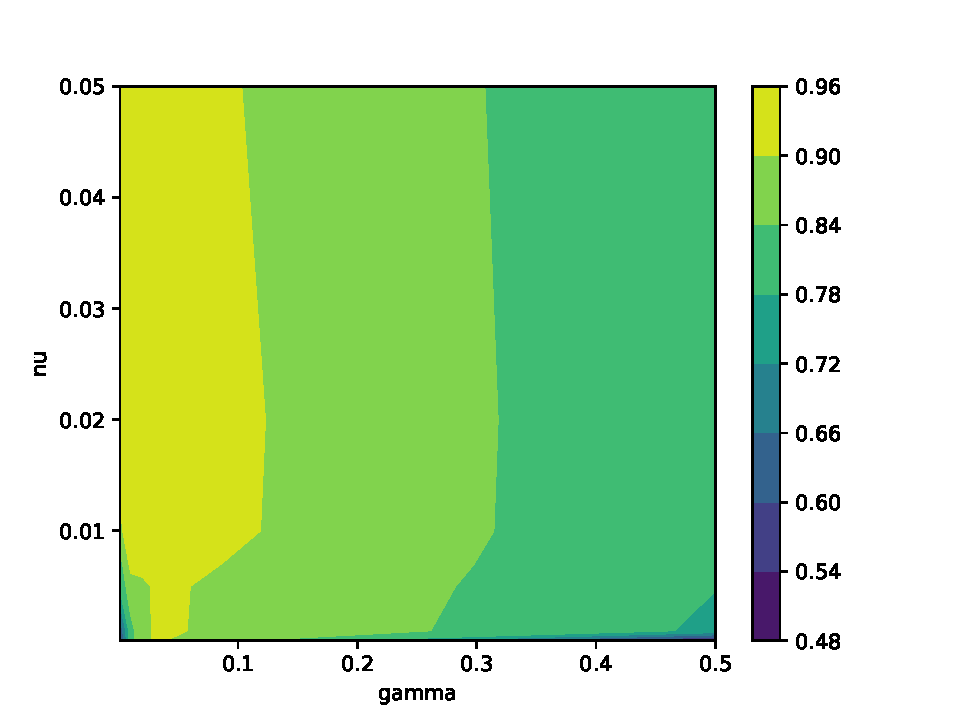
\includegraphics[width=\textwidth]{images/ocsvm-accuracy.pdf}
        \caption{OCSVM Accuracy}
    \end{minipage}
    \hfill
    \begin{minipage}[t]{0.5\textwidth}
        \vspace{0pt}
        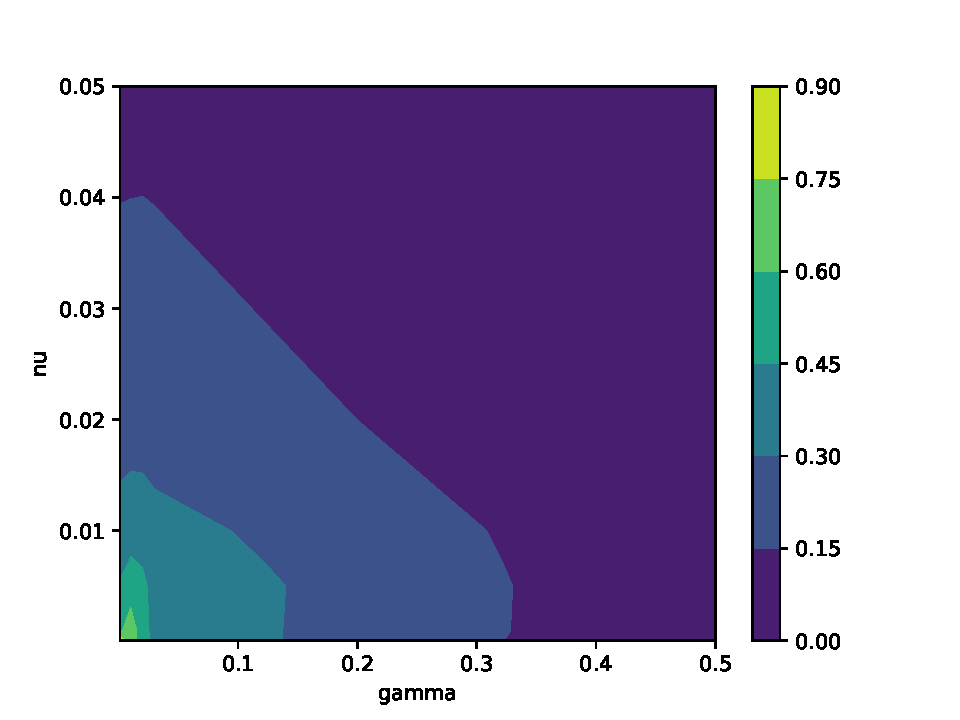
\includegraphics[width=\textwidth]{images/ocsvm-precision.pdf}
        \caption{OCSVM Precision}
    \end{minipage}
    \\
    \begin{minipage}[t]{0.5\textwidth}
        \vspace{0pt}
        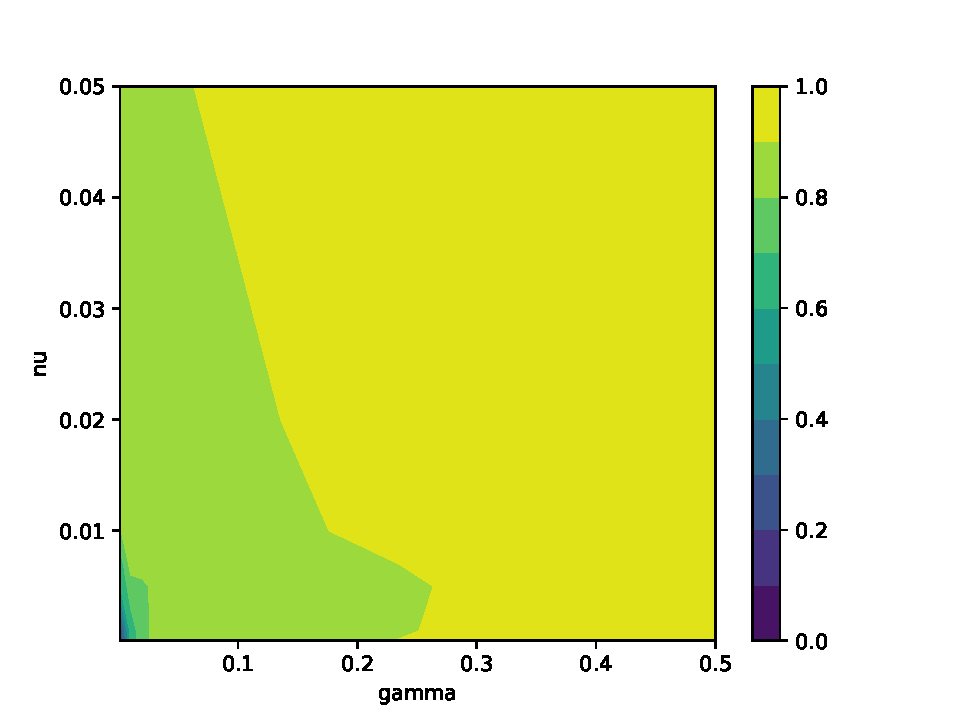
\includegraphics[width=\textwidth]{images/ocsvm-recall.pdf}
        \caption{OCSVM Recall}
    \end{minipage}
    \hfill
    \begin{minipage}[t]{0.5\textwidth}
        \vspace{0pt}
        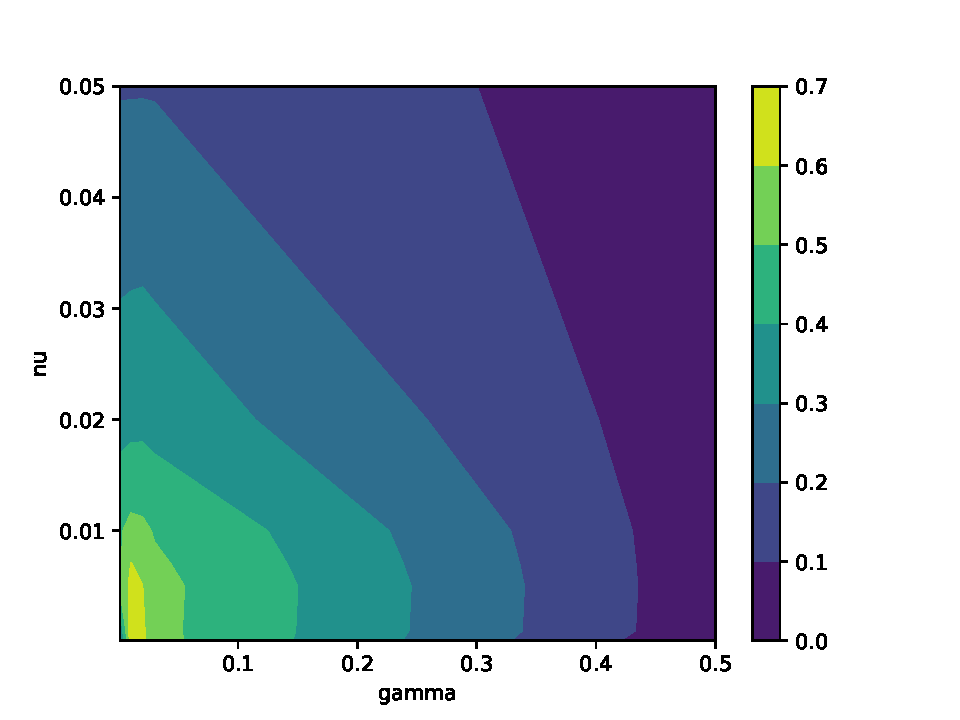
\includegraphics[width=\textwidth]{images/ocsvm-f1.pdf}
        \caption{OCSVM F1 score}
    \end{minipage}
\end{figure}

\noindent

\subsection{Gaussian Mixture Model}

\begin{table}[H]
  \centering
  \begin{tabularx}{\textwidth}{
      |X
      |X
      |X
      |X
      |X
      |X|
  }
  \hline
  $K$ & $q$ & {Accuracy} & {Recall} & {Precision} & {F1 Score} \\
  \hline
  \rowcolor{gray!20} 4 & 0.01 & 0.920 & 0.845 & 0.581 & 0.688  \\
  3	& 0.01 & 0.918	& 0.841 & 0.578 & 0.685 \\
  \rowcolor{gray!20} 2	& 0.01 & 0.918 & 0.841 & 0.578	& 0.685  \\
  1 & 0.01 & 0.914 & 0.833 & 0.572 & 0.678 \\
  \rowcolor{gray!20} 5 & 0.01 & 0.912	& 0.829 & 0.569	& 0.675  \\
  \hline
  \end{tabularx}
  \caption{Cele mai bune rezultate, în funcţie de F1, obţinute pentru Gaussian Mixture Model}
\end{table}



Pentru acest model, hiperparametrul optim 
căutat este numărul de componente Gaussiene $K$. Vom încerca pe rând fiecare valoare
din $K\in\{1, 2, 3, \ldots, 16, 17\}$. De asemenea, pentru că modelul 
ne va oferi probabilitățile de apartenență a unui punct pentru 
fiecare componentă, vom avea nevoie și de un prag pentru a decide 
dacă punctul este sau nu anomalie. Ne vom folosi de cuantile 
calculate pe setul de validare pentru a găsi pragul optim.

Pentru $K=1$ putem afla parametrii foarte eficient folosind 
\textbf{Maximum Likelihood Estimation}, întrucât problema 
se reduce la aflarea mediei şi a matricei de 
covarianţă pentru o distribuţie Gaussiană. 

Pentru $K > 1$ vom folosi \textbf{Expectation Maximization} 
pentru a găsi parametrii optimi, 
având în vedere ca numărul de componente este precizat de la început.

Gaussian Mixture Model încearcă să estimeze o distribuţie posibil multimodală 
folosind mai multe componente Gaussiene. Prin urmare, numărul optim de componente
ne indică intuitiv numărul de \textbf{moduri} pe care le are distribuţia ce a generat 
setul de date.
Se observă că modelul se descurcă destul de bine chiar şi cu o singură componentă. 
Aceasta ne indică faptul ca distribuţia ce a generat setul de date este 
similară cu una Gaussiană.

Pentru acest model, pragul este foarte important. Dacă avem acelaşi prag,
dar număr de componente diferite, varianţa rezultatelor
nu este prea mare, dar dacă alegem greșit valoarea cuantilei, 
performanţa modelului are de suferit. Totuşi, 
dată simplitatea modelului, rezultatele sunt impresionante.
Cu un timp de antrenare de sub câteva minute, obține rezultate 
mai bune decât One Class SVM pe setul de validare.

Alegem \textbf{numărul de componente $K=4$} şi valoarea
cuantilei $q=0.01$ pentru modelul final, chiar dacă 
am avut rezultate bune şi cu $K=1$ deoarece ne dorim un model puţin mai complex 
decât o banală distribuţie Gaussiană. În practică, este o şansă mică să dăm peste 
un proces care să genereze date fix în acest mod. De asemenea, aici F1 score are valoarea cea mai mare
şi după aceasta ne vom ghida, având în vedere că ne interesează performanţa modelului 
per total.

\begin{figure}[!htb] % Use a separate page for the figure
    \begin{minipage}[t]{0.5\textwidth}
        \vspace{0pt}
        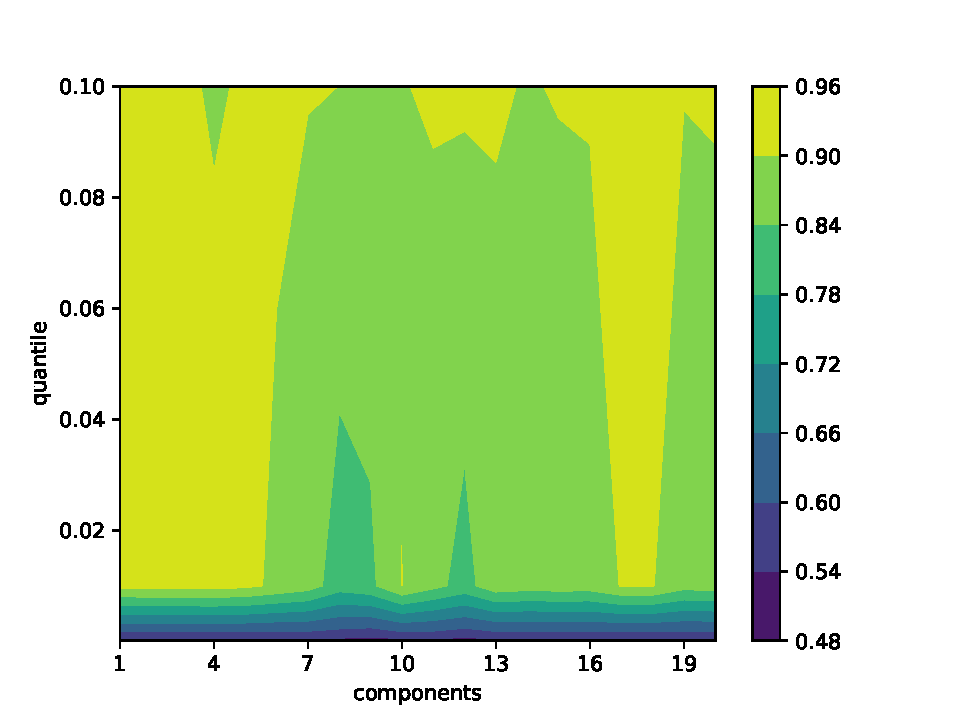
\includegraphics[width=\textwidth]{images/gmm-accuracy.pdf}
        \caption{GMM Accuracy}
    \end{minipage}
    \hfill
    \begin{minipage}[t]{0.5\textwidth}
        \vspace{0pt}
        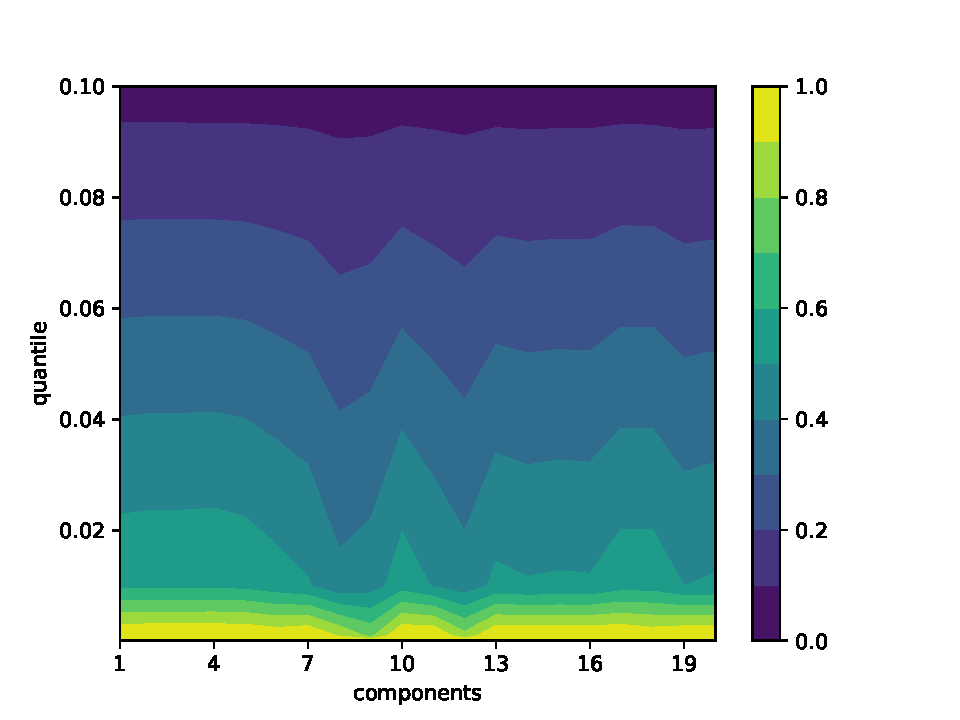
\includegraphics[width=\textwidth]{images/gmm-precision.pdf}
        \caption{GMM Precision}
    \end{minipage}
    \\
    \begin{minipage}[t]{0.5\textwidth}
        \vspace{0pt}
        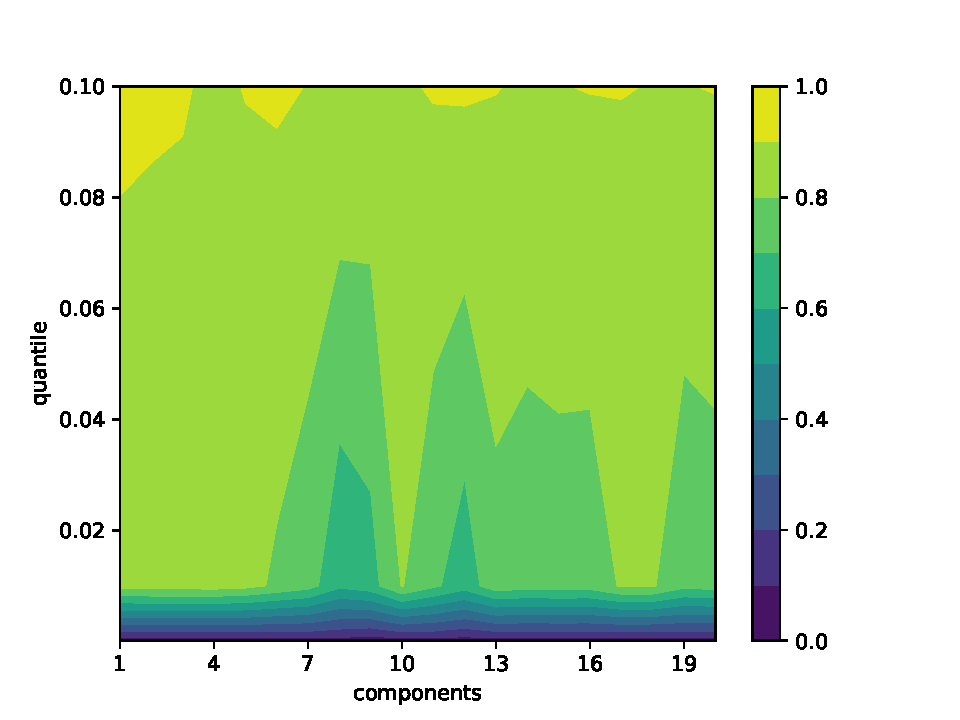
\includegraphics[width=\textwidth]{images/gmm-recall.pdf}
        \caption{GMM Recall}
    \end{minipage}
    \hfill
    \begin{minipage}[t]{0.5\textwidth}
        \vspace{0pt}
        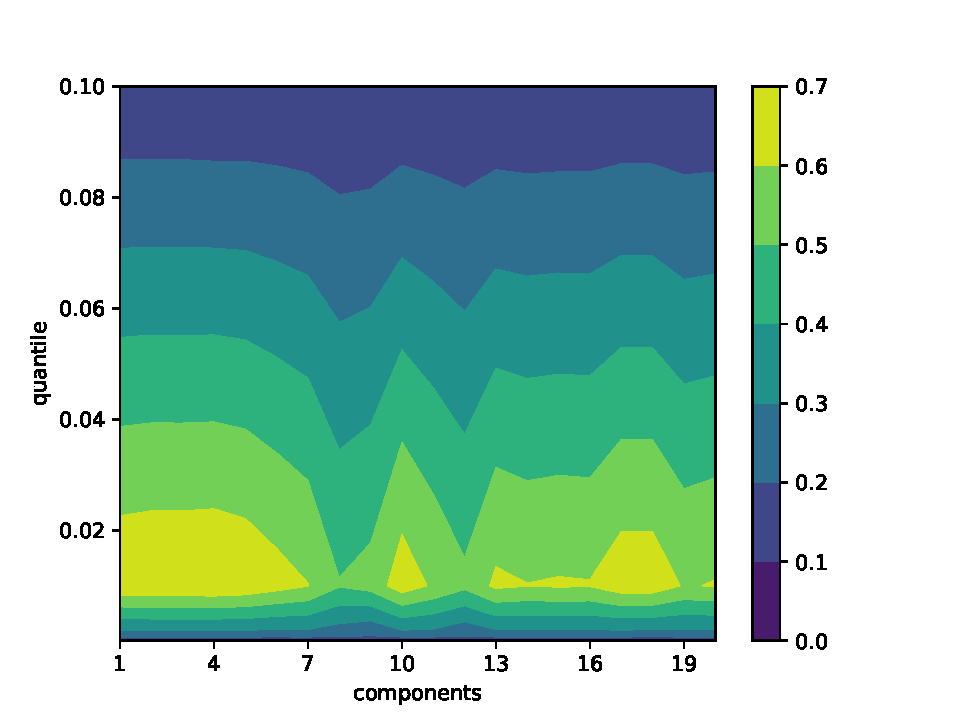
\includegraphics[width=\textwidth]{images/gmm-f1.pdf}
        \caption{GMM F1 score}
    \end{minipage}
\end{figure}

\noindent
  

\subsection{Kernel Density Estimation}

\begin{table}[H]
  \centering
  \begin{tabularx}{\textwidth}{
      |X
      |X
      |X
      |X
      |X
      |X
      |X
      |X|
  }
  \hline
  $Kernel$ & $h$ & $q$ & {Accuracy} & {Recall} & {Precision} & {F1 Score} \\
  \hline
  \rowcolor{gray!20} tophat	& 9	& 0.01 & 0.908 & 0.821 & 0.562 & 0.667  \\
  linear & 9 & 0.01	& 0.881 & 0.768	& 0.527 & 0.625 \\
  \rowcolor{gray!20} parabolic & 9 & 0.01 & 0.877 & 0.760 & 0.522 & 0.619  \\
  cosine & 9 & 0.01	& 0.875 & 0.756	& 0.519 & 0.615 \\
  \rowcolor{gray!20} tophat	& 8	& 0.01 & 0.877 & 0.760 & 0.513 & 0.613 \\
  \hline
  \end{tabularx}
  \caption{Cele mai bune rezultate, în funcţie de F1, obţinute pentru Kernel Density Estimation}
\end{table}

Am testat mai multe funcţii kernel, anume: \textbf{tophat}, 
\textbf{liniar}, \textbf{parabolic}, \textbf{cosinus},
\textbf{exponenţial} şi \textbf{gaussian}. 
Deşi kernelul Gaussian este cel mai des întâlnit în practică
datorită numeroaselor proprietăţi utile pe care le deţine, aici se observă
că nu obține rezultate satisfăcătoare, kernelul \textbf{tophat}
fiind cel care performează
cel mai bine. De asemenea, trebuie 
să impunem un prag după care să decidem daca un punct este sau nu anomalie. 
Vom alege cuantile luate pe setul de validare, precum în cazul 
Gaussian Mixture Model.

Lăţimea de bandă este cea care stă la baza \textbf{bias-variance tradeoff} 
în acest model.
Valorile prea mici implică \textbf{variance} mare, întrucât aria de sub grafic 
pentru fiecare punct este influenţată doar de punctele foarte apropiate de el, 
fapt ce duce la o distribuţie cu mulţi "ţepi". 
În schimb, valorile prea mari implică \textbf{bias} mare pentru că acum şi punctele 
aflate la distanţă mare joacă un rol important. În cel mai rău caz, o distribuţie 
multimodală ajunge sa fie estimată ca una unimodală din cauza netezimii graficului.

Se observă că modelul are o performanţă mai bună pentru valori 
mai mari ale lăţimii de banda, indiferent de kernel. Totuşi, 
la fel de importantă este şi cuantila pentru obţinerea rezultatelor 
cele mai bune. Acest lucru este ilustrat și pe graficele de mai jos. 
Spre deosebire de Gaussian Mixture Model, cuantila 
folosită nu are un puternic impact asupra performanţei modelului de una singură.

Din păcate, după un timp de antrenare ce depășește 40 minute, 
timp ce se află între valorile pentru OCSVM și GMM, nu obținem 
rezultate mai bune decât GMM
pe setul de validare. 

Alegem \textbf{lăţimea de bandă} $h=9$, kernelul \textbf{tophat} şi valoarea
cuantilei $q=0.01$ pentru modelul final deoarece are cea
mai bună valoare pentru F1 score.

\begin{figure}[!htb] % Use a separate page for the figure
    \begin{minipage}[t]{0.5\textwidth}
        \vspace{0pt}
        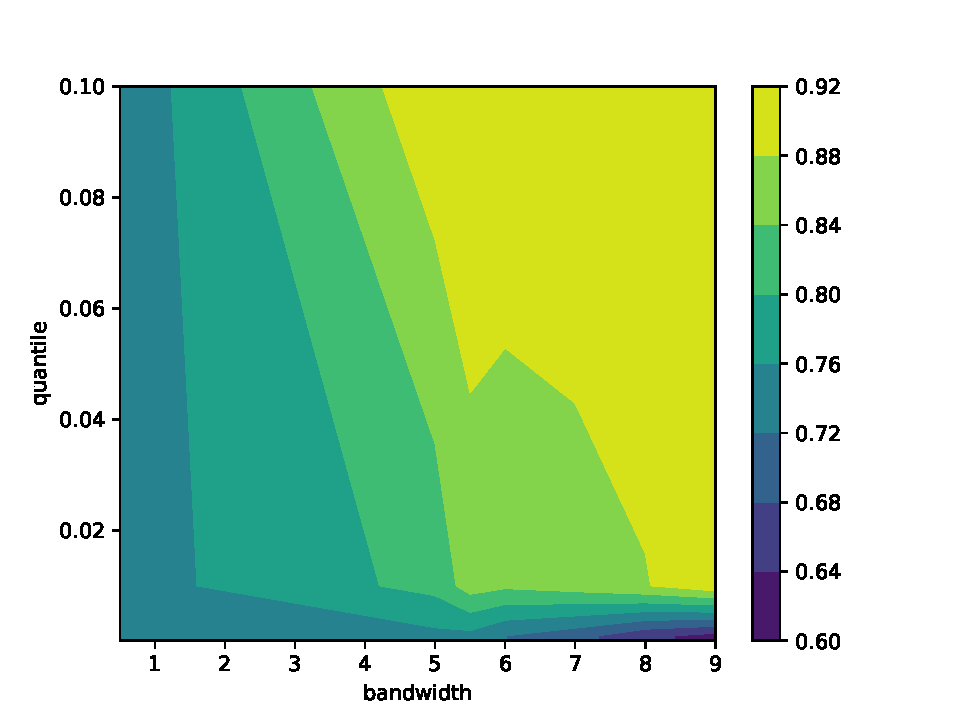
\includegraphics[width=\textwidth]{images/kde-accuracy.pdf}
        \caption{KDE Accuracy}
    \end{minipage}
    \hfill
    \begin{minipage}[t]{0.5\textwidth}
        \vspace{0pt}
        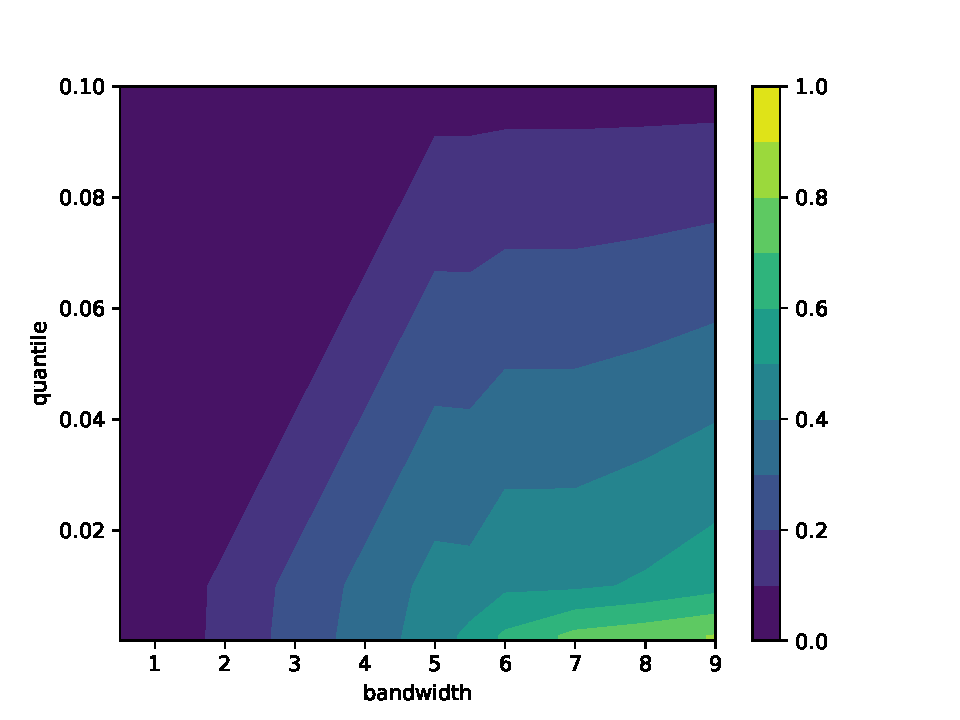
\includegraphics[width=\textwidth]{images/kde-precision.pdf}
        \caption{KDE Precision}
    \end{minipage}
    \\
    \begin{minipage}[t]{0.5\textwidth}
        \vspace{0pt}
        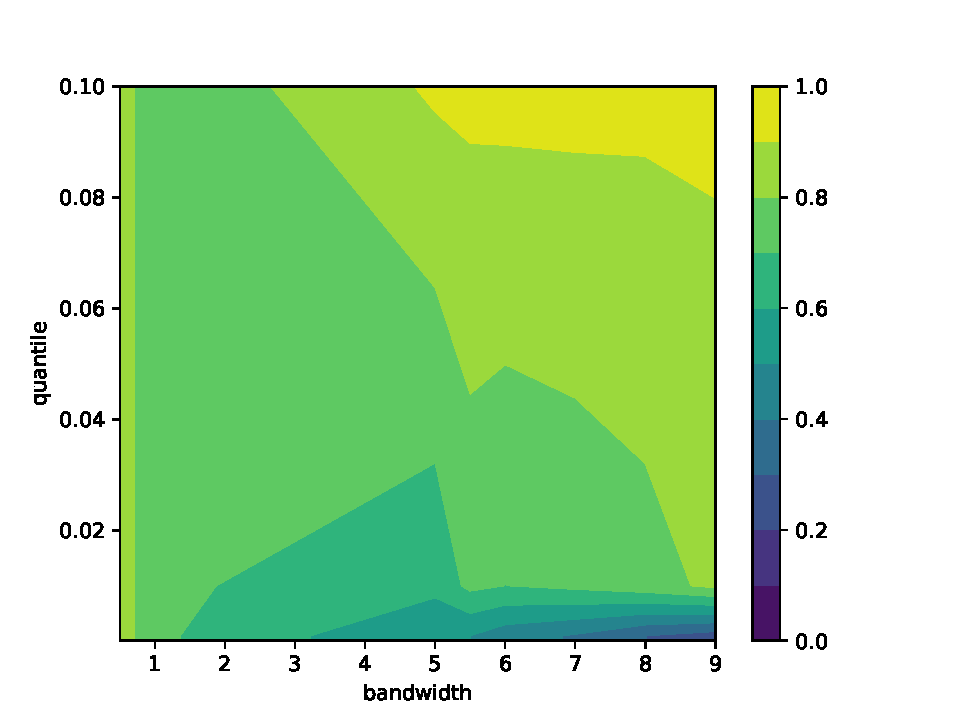
\includegraphics[width=\textwidth]{images/kde-recall.pdf}
        \caption{KDE Recall}
    \end{minipage}
    \hfill
    \begin{minipage}[t]{0.5\textwidth}
        \vspace{0pt}
        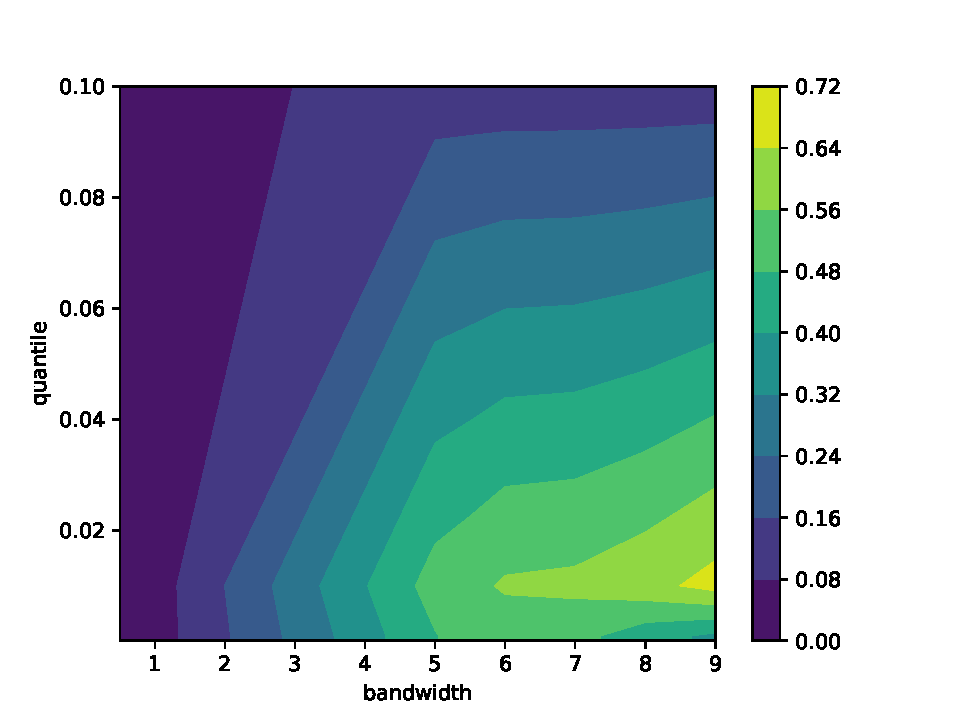
\includegraphics[width=\textwidth]{images/kde-f1.pdf}
        \caption{KDE F1 score}
    \end{minipage}
\end{figure}

\noindent

\section{Modele supervizate}

\subsection{SVM Supervizat}

Pentru a profita de faptul că avem la dispoziţie etichetele datelor, vom trata 
problema şi din punct de vedere supervizat. Scopul acestui experiment
este de a vedea impactul etichetelor asupra performanţei algoritmilor, 
comparând cazul ideal, unde putem folosi metode supervizate, cu cel din lumea reală,
unde, de obicei, ne bazăm pe cele nesupervizate în lipsa etichetelor.

Gaussian Mixture Model şi Kernel 
Density Estimation nu pot fi aplicate decât într-un mediu nesupervizat, aşa 
că vom antrena doar SVM-ul, dar de data aceasta pentru clasificare binară.
Astfel, putem observa performanţa algoritmilor prezentaţi anterior şi faţă 
de un algoritm supervizat care are de rezolvat o problemă relativ mai uşoară.

O modificare pe care o vom face la modul de împărţire al setului de date 
este că de această dată stratificarea este luată în calcul, aşa că păstrăm 
ponderile claselor aproximativ la fel în toate cele 3 partiţii.

Şi aici, kernel-ul Gaussian este cel care oferă cele mai bune rezultate cu 
valori scăzute pentru $\gamma$, similar cu cazul OCSVM, dar parametrul 
$\nu$ este înlocuit
de parametrul $C$ care are rolul de regularizare în SVM-ul Soft-Margin.

Se observă o creştere substanţială a valorilor metricilor atunci când tratăm 
problema în mod supervizat, \textbf{F1 Score} 
depăşind 0.87 pe setul de validare, în timp ce 
OCSVM pe setul de validare abia atingea 0.66.

\begin{table}[H]
    \centering
    \begin{tabularx}{\textwidth}{
        |X
        |X
        |X
        |X
        |X
        |X|
    }
    \hline
    $\gamma$ & $C$ & {Accuracy} & {Recall} & {Precision} & {F1 Score} \\
    \hline
    \rowcolor{gray!20} 0.01 & 0.1 & 0.7972 & 0.5946 & 0.8302 & 0.6929 \\
    0.01 & 0.5 & 0.9053 & 0.8108 & 0.8571 & 0.8333 \\
    \rowcolor{gray!20} 0.01 & 1.0 & 0.9053 & 0.8108 & 0.8824 & 0.8451 \\
    0.01 & 2.0 & 0.9053 & 0.8108 & 0.8955 & 0.8511 \\
    \rowcolor{gray!20} 0.01 & 3.0 & 0.9054 & 0.8108 & 0.9375 & 0.8696 \\
    \rowcolor{red!40} 0.01 & 4.0 & 0.9054 & 0.8108 & 0.9524 & 0.8759 \\
    \rowcolor{gray!20} 0.02 & 0.1 & 0.7094 & 0.4189 & 0.7750 & 0.5439 \\
    0.02 & 0.5 & 0.8850 & 0.7703 & 0.8769 & 0.8201 \\
    \rowcolor{gray!20} 0.02 & 1.0 & 0.8918 & 0.7838 & 0.9355 & 0.8529 \\
    0.02 & 2.0 & 0.8919 & 0.7838 & 0.9508 & 0.8593 \\
    \rowcolor{gray!20} 0.02 & 3.0 & 0.8919 & 0.7838 & 0.9508 & 0.8593 \\
    0.02 & 4.0 & 0.8919 & 0.7838 & 0.9667 & 0.8657 \\
    \rowcolor{gray!20} 0.03 & 0.1 & 0.6148 & 0.2297 & 0.8947 & 0.3656 \\
    0.03 & 0.5 & 0.8243 & 0.6486 & 0.9412 & 0.7680 \\
    \rowcolor{gray!20} 0.03 & 1.0 & 0.8783 & 0.7568 & 0.9492 & 0.8421 \\
    0.03 & 2.0 & 0.8851 & 0.7703 & 0.9661 & 0.8571 \\
    \rowcolor{gray!20} 0.03 & 3.0 & 0.8851 & 0.7703 & 0.9661 & 0.8571 \\
    0.03 & 4.0 & 0.8851 & 0.7703 & 0.9661 & 0.8571 \\
    \hline
    \end{tabularx}
    \caption{Grid Search pentru SVM}
\end{table}
  